\setRL
%\pagenumbering{arabic} 


انرژی انحنای غشا بدون در نظر گرفتن قید سطحی و حجمی با انرژی هلفریش 
\cite{Helfrich1973}
توصیف می‌شود. انرژی خمش معمولا به شکل زیر بازنویسی می‌شود،
\begin{equation}
E_{b}=\frac{1}{2}\kappa\int dS\left(H-H_0\right)^2
\label{eq:HelfrichBendingEnergyH}
\end{equation}
که در آن
\begin{equation}
\begin{aligned}
H=C_1+C_2\\
H_0=2C_0
\end{aligned}
\end{equation}

و با معادله‌ی 
\ref{eq:HelfrichBendingEnergy}
برابر است. شکل
\ref{fig:undulatedCircle}
سطح یک غشای کُروی را نمایش می‌دهد که شعاع متوسط 
$r_0$
دارد. مانند مثال ریسمان که در مقدمه مطح شد، ما می‌توانیم شکل پیچیده‌ی برآمدگی‌ها و فرو رفتگی‌ها (خط آبی رنگ در شکل 
\ref{fig:undulatedCircle}
) را بر حسب مُد‌های نرمال آن بنویسیم. به علت هندسه‌ی مسئله انتخاب دستگاه مختصات کُروی محاسبات را ساده‌تر خواهد کرد. مُد‌های نرمال در مختصات کُروی هماهنگ‌های کروی
\LTRfootnote{spherical harmonics}
هستند که با حل معادله‌ی پواسون در این دستگاه مختصات محاسبه می‌شود. 
\begin{figure}[h]
\begin{center}
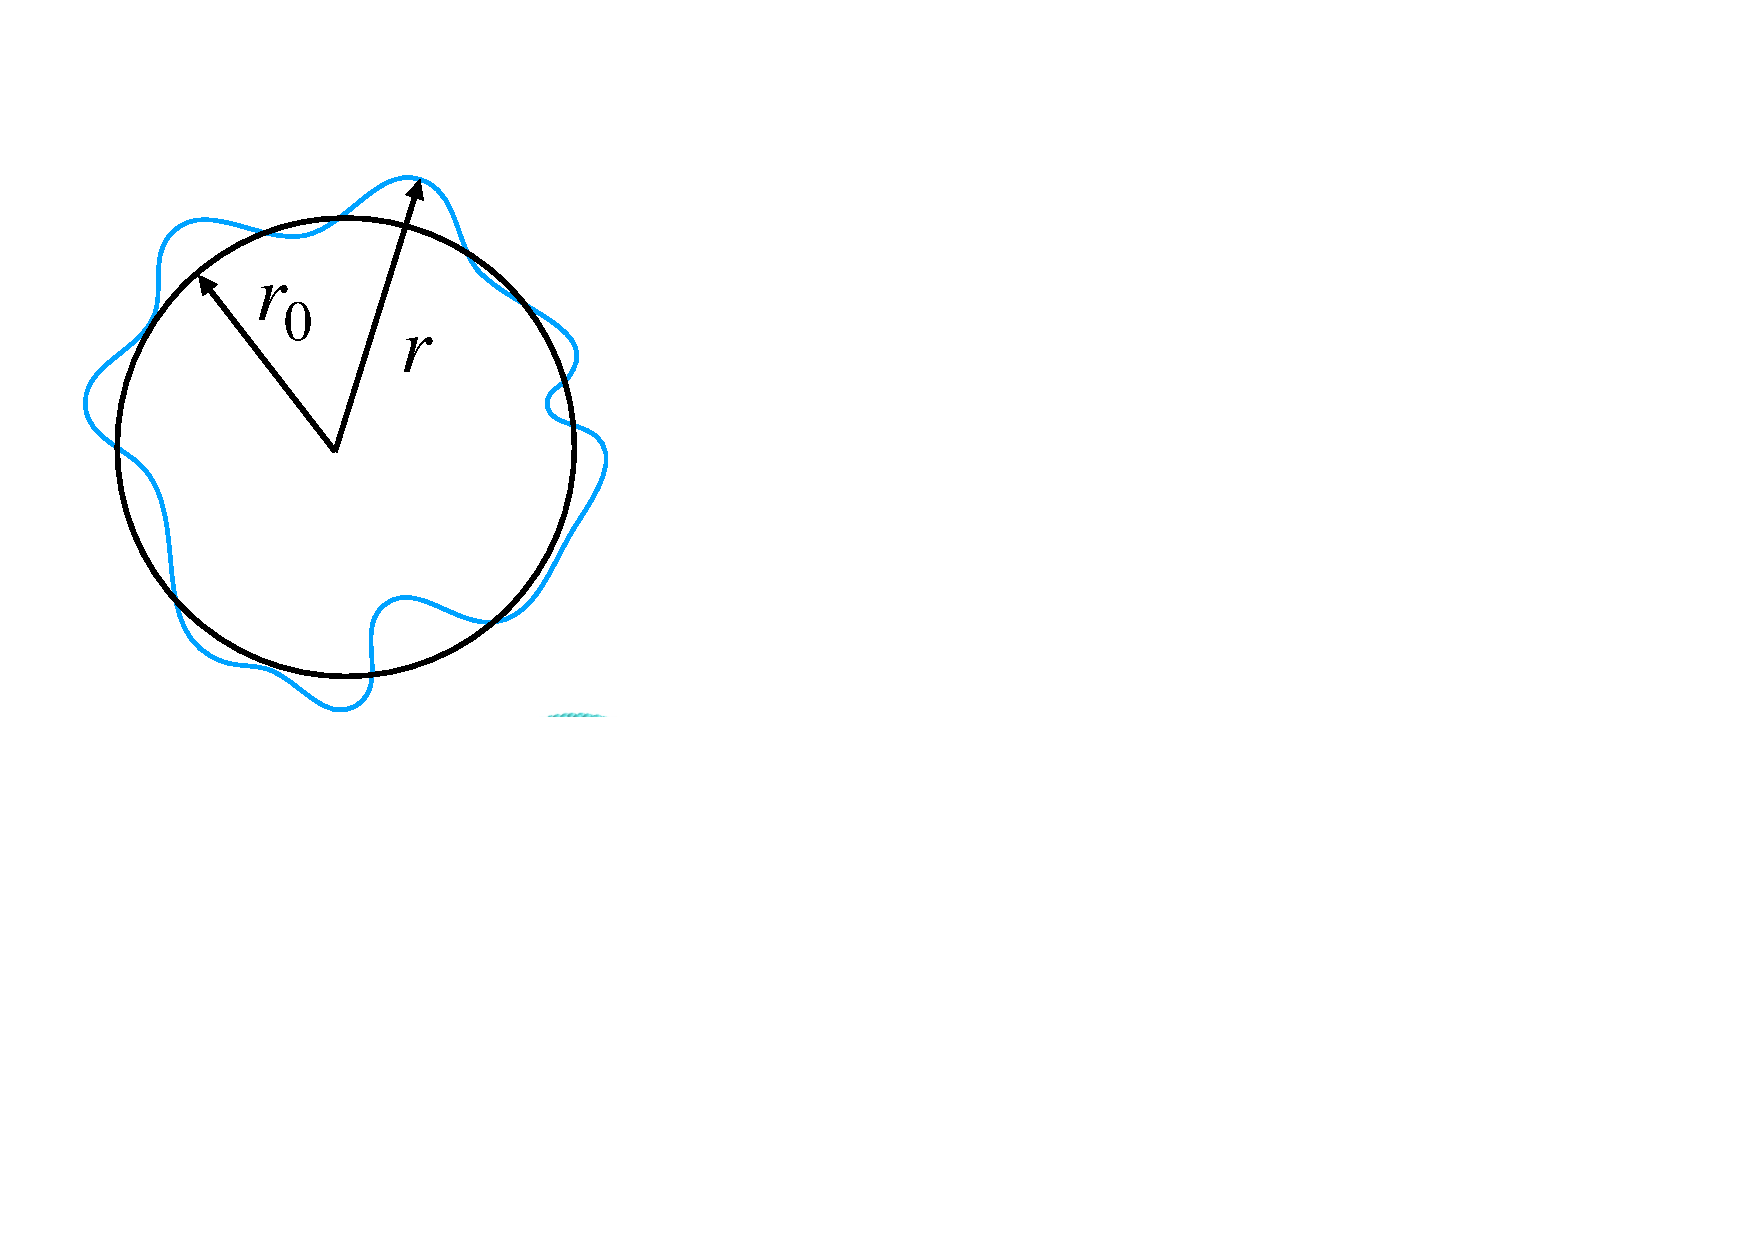
\includegraphics[width=4.5in]{\MemFluc /Pics/undulatedCircle}
\caption{
یک ترسیم از سطح مقطع یک غشای کُروی شکل با شعاع متوسط 
$r_0$
(خط مشکل) و برآمدگی و فرورفتگی‌های روی سطح آن (خط آبی رنگ). مکان هر نقطه روی سطح با بردار 
$\vec r$
نمایش داده می‌شود.
}
\label{fig:undulatedCircle}
\end{center}
\end{figure}
در نتیجه هر نقطه روی سطح کُره را بر حسب شعاع متوسط کُره و به شکل زیر بیان کرد،
\begin{equation}
r(\theta,\phi)=r_0\left[1+g(\theta,\phi)\right]
\end{equation}
که 
$g(\theta,\phi)$
بسط بر حسب مُدهای کُروی است،
\begin{equation}
g(\theta,\phi)=\sum_{\ell,m}u_{\ell m}Y_{\ell m} (\theta,\phi).
\label{eq:gdef}
\end{equation}
و تعریف هماهنگ‌های کروی بر حسب تابع لژاندر
\LTRfootnote{Legandre polynomials}
$P_\ell^m(x)$
به شکل
\begin{equation}
Y_{\ell,m}(\theta,\phi)=\sqrt{\frac{2\ell+1}{4\pi}}\sqrt{\frac{(\ell-|m|)!}{(\ell+|m|)!}}~P_\ell^m(\cos\theta)~e^{im\phi}.
\label{eq:rYlmLogandre}
\end{equation}
است و 
$u_{\ell,m}$
شدت هر مُد را مشخص می‌کند. رابطه‌ی تعامدی هماهنگ‌های کروی به شکل انتگرال سطحی زیر تعریف می‌شود،
\begin{equation}
\int d\Omega~Y_{\ell,m}(\theta,\phi)Y_{\ell',m'}(\theta,\phi)=\delta_{\ell,\ell'}\delta_{m,m'}
\label{eq:rYlmOrthonormal}
\end{equation}


مُد‌های کُروی تغییر شکل کره را نشان می‌دهند (به شکل 
\ref{fig:ulmExamples}
توجه کنید).
\begin{figure}[h]
\begin{center}
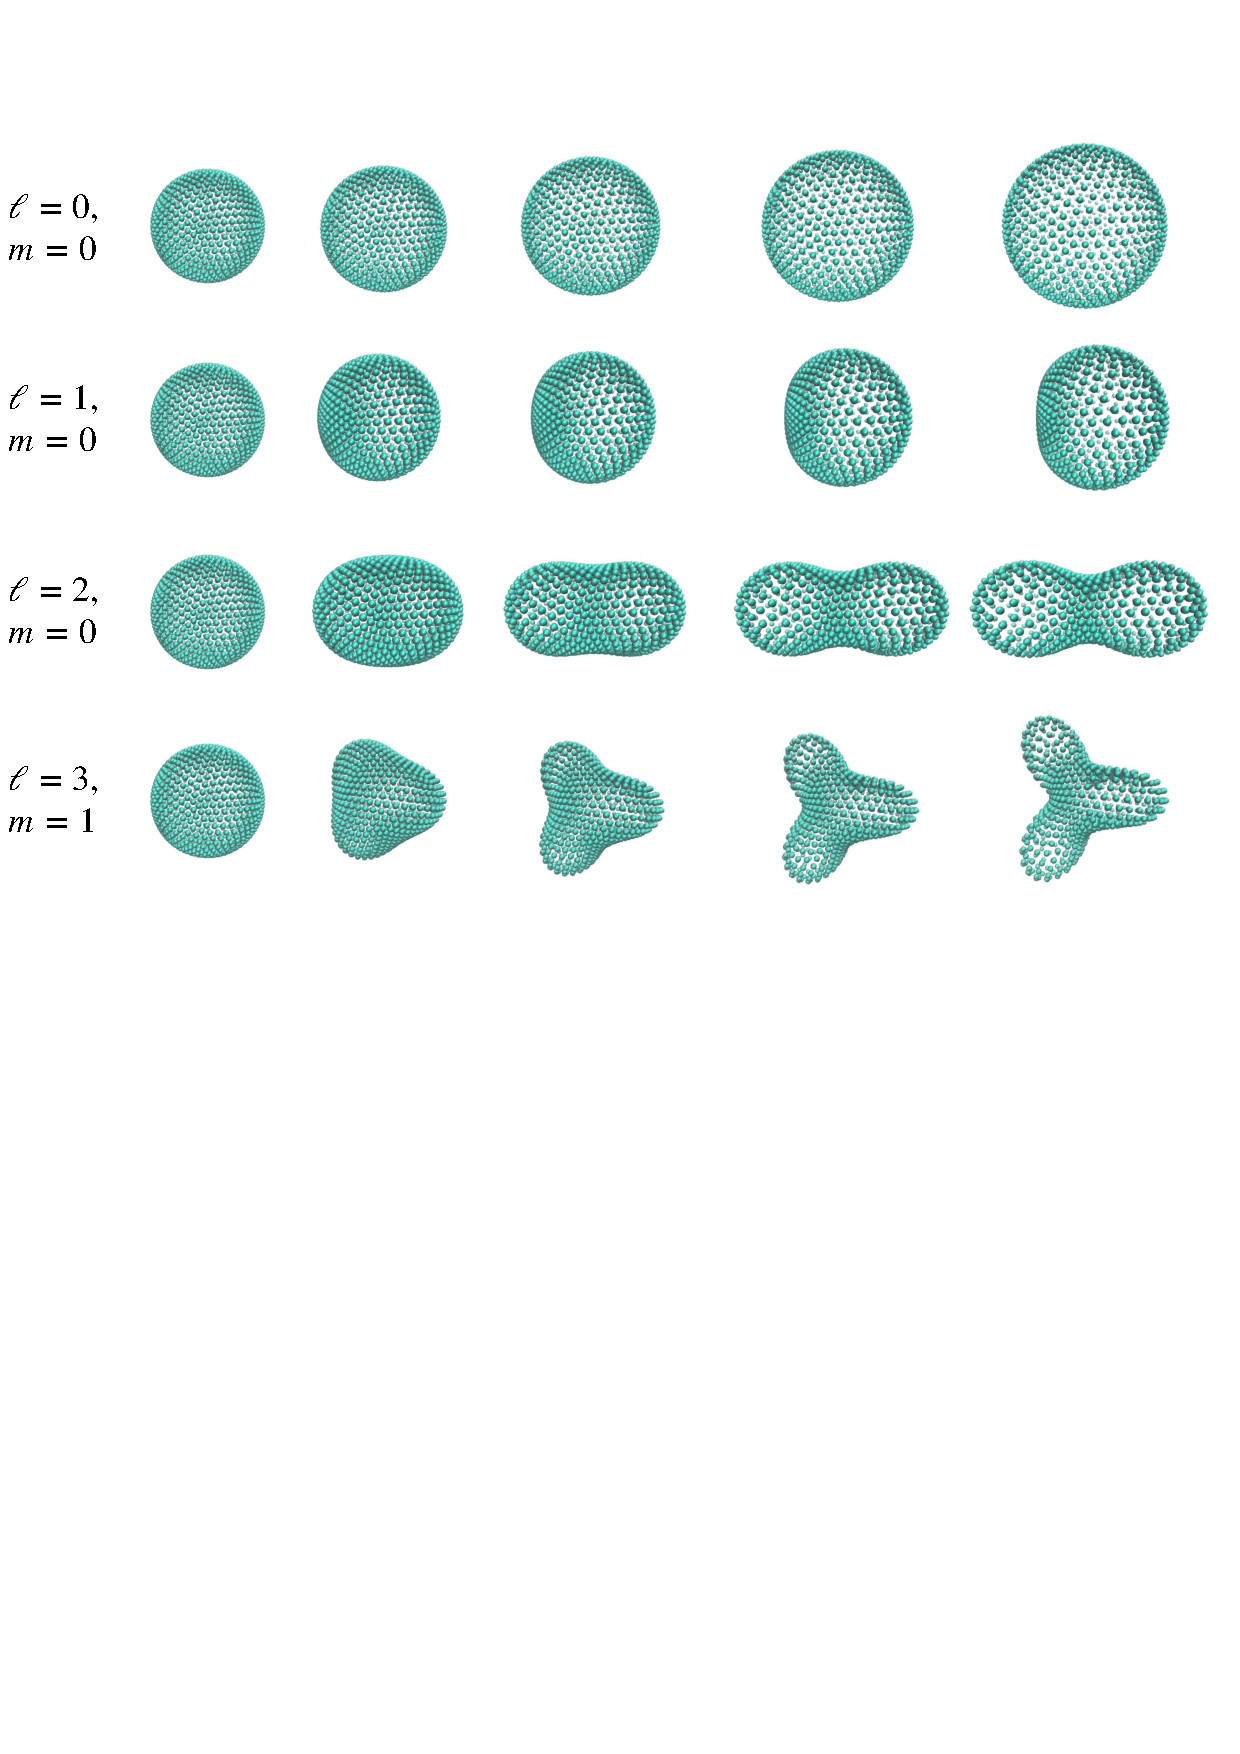
\includegraphics[width=6in]{\MemFluc /Pics/modeExamples}
\caption{
در این شکل در هر ردیف نحوه‌ی تغییر شکل یک کُره بر اثر افزودن یک جمله‌ی 
$Y_{\ell,m}$
را نشان می‌دهد که از چپ به راست شدّت مُد
$u_{\ell,m}$
افزایش یافته‌است. مُد‌ 
$Y_{0,0}$
اثر تغییر حجم کُره را نشان می‌دهد. مُد‌های 
$Y_{1,m}$
که با سه 
$m=-1,0,1$
متمایز می‌شوند، برای شدّت‌های کوچک جابجایی فضایی در راستا‌های 
$x,y,z$
را مشخص می‌کنند. مُد
$Y_{2,m}$
اولین مُدی‌است که تغییر شکل اساسی کُره را نشان می‌دهد. در شکل بالا برای مثال مُد
$m=0$
رسم شده‌است. مُدهای بالاتر نیز تغییر شکل‌های پیچیده‌تری را مشخص می‌کنند که در اینجا برای مثال مُد 
$Y_{3,1}$
نمایش داده شده‌است. جهت بهتر نمایش دادن تغییر شکل مُدها میزان شدّت مُد برای ردیف‌های مختلف در بازه‌های مختلف انتخاب شده‌است.
}
\label{fig:ulmExamples}
\end{center}
\end{figure}

در این شکل تاثیر مُدهای مختلف در تغییر شکل یک کُره را با چند مثال نشان می‌دهد. همانطور که می‌دانید عدد مُد 
$m$
مقادیر صحیح بین 
$-\ell<m<\ell$
را اختیار می‌کند.  مُد
$Y_{0,0}$
کاملا متقارن است و شدّت آن تغییرات شعاع کفره را مشخص می‌کند. از طرفی در حد شدّت کوچک، مُد 
$Y_{1,m}$
(بسته به مقدار 
$m=-1,0,1$
) جابجایی فضایی کُره در سه جهت اصلی فضا 
$x,y$
و
$z$
را نشان می‌دهد. سری مُدهای 
$Y_{2,m}$
کوچک‌ترین عدد مُدی است که در واقع «تغییر شکل» از حالت کُروی را نشان می‌دهد. مُدهای بالاتر تغییر شکل‌های پیچیده‌تری را نمایش می‌دهند. در شرایط شدّت مُد
$u_{\ell,m}$
یکسان مُدهای
$Y_{2,m}$
بیشترین تغییر شکل کُره را مشخص کرده و با افزایش عدد مُد تغییر شکل روند نزولی دارد.


با فرض اینکه خمش ذاتی در تمام نقاط کُره و در تمام جهت‌ها یکسان است و مقدار 
$r_s$
دارد معادله‌ی
\ref{eq:HelfrichBendingEnergyH}
را می‌توانیم بر حسب دیورژانس بردار عمود بر سطح در نقطه به شکل زیر بنویسیم
\cite{safran1983}
\begin{equation}
E_{b}=\frac{1}{2}\kappa\int dS\left(\nabla\cdot\hat n-\frac{2}{r_s}\right)^2
\label{eq:ebforsubstitution}
\end{equation}

که در معادله‌ی بالا رابطه‌ی خمش میانگین با بردار عمود بر سطح به این گونه تعریف می‌شود،
\begin{equation}
H=(C_1+C_2)=\left(\frac{1}{r_1}+\frac{1}{r_2}\right)=\nabla\cdot\hat n.
\end{equation}
‌ در معادله بالا
$r_1$ و $r_2$
شعاع‌های اصلی خمش
\LTRfootnote{principle curvature radii}
و $\hat n$ بردار عمود بر سطح است.

در نتیجه می‌توانیم معادله‌ی سطح تقریبا کروی که مرکز آن در مبدا مختصات وجود دارد را به شکل زیر تعریف می‌کنیم
\begin{equation}
R(r)= r-r_0\left[1+g(\theta,\phi)\right]=0
\label{eq:radiusdef}
\end{equation}
که اختلاف شعاع هر نقطه از شعاع متوسط است. بردار عمود در هر نقطه از سطح کره را می‌توانیم به شکل گرادیان معدله‌ی سطح محاسبه کنیم
\begin{equation}
\hat n = \frac{\nabla R(r)}{|\nabla R(r)|}= \frac{\hat r-\frac{r_0}{r}g_\theta \hat\theta-\frac{r_0}{r\sin\theta}g_\phi\hat\phi }{\sqrt{1+\left(\frac{r_0}{r}g_\theta\right)^2+\left(\frac{r_0}{r\sin\theta}g_\phi\right)^2 }}
\end{equation}
که در اینجا برای ساده سازی از
$g_\theta=\partial/\partial\theta g$
و
$g_\phi=\partial/\partial\phi g$
استفاده شده‌است و محاسبات در دستگاه مختصات کروی انجام شده‌است.
جهت یادآوری،
\begin{equation}
\begin{aligned}
&\nabla f =\frac{\partial}{\partial r}f\hat r + \frac{1}{r} \frac{\partial}{\partial\theta}f\hat\theta+ \frac{1}{r\sin\theta} \frac{\partial}{\partial\phi}f\hat\phi\\
&\nabla\cdot \vec A =\frac{1}{r^2}\frac{\partial}{\partial r}(r^2A_r)+ \frac{1}{r\sin\theta} \frac{\partial}{\partial\theta}(A_\theta\sin\theta)+ \frac{1}{r\sin\theta} \frac{\partial}{\partial\phi}A_\phi\\
&\nabla^2f =\frac{1}{r^2}\frac{\partial}{\partial r}\left(r^2\frac{\partial}{\partial r}f\right)+ \frac{1}{r^2\sin\theta} \frac{\partial}{\partial\theta}\left(\sin\theta\frac{\partial}{\partial\theta}f\right)+ \frac{1}{r^2\sin^2\theta} \frac{\partial^2}{\partial\phi^2}f
\end{aligned}
\end{equation}
از این پس محاسبات را تنها تا مرتبه‌ی دوم نسبت به $g$ 
انجام خواهیم داد. در نتیجه بردار عمود بر سطح را به این شکل بازنویسی می‌کنیم،
\begin{equation}
\hat n \simeq\left\{1-\frac{1}{2}\left[\left(\frac{r_0}{r}g_\theta\right)^2+\left(\frac{r_0}{r\sin\theta}g_\phi\right)^2 \right]\right\}^{-\frac{1}{2}}\left( \hat r-\frac{r_0}{r}g_\theta \hat\theta-\frac{r_0}{r\sin\theta}g_\phi\hat\phi \right)
\end{equation}
حالا می‌توان دیورژانس را به ترتیب زیر محاسبه کرد،
\begin{equation}
\begin{aligned}
&\nabla\cdot\hat n \simeq \frac{2}{r}+\frac{1}{r\sin\theta}\frac{\partial}{\partial\theta}\left(-\frac{r_0}{r}g_\theta\sin\theta\right)+\frac{1}{r\sin\theta}\left(-\frac{r_0}{r\sin\theta}g_\phi\right)\\
&=\frac{2}{r}\left[1-\frac{r_0}{2r}\left(\frac{1}{\sin\theta}\frac{\partial}{\partial\theta}g_\theta\sin\theta+\frac{1}{\sin^2\theta}g_{\phi\phi}\right)\right]
\label{eq:divn}
\end{aligned}
\end{equation}
با در نظر گرفتن تعریف عملگر اندازه حرکت زاویه‌ای 
\begin{equation}
L^2=-\frac{1}{\sin\theta}\frac{\partial}{\partial\theta}\left(\sin\theta\frac{\partial}{\partial\theta}\right)-\frac{1}{\sin^2\theta}\left(\frac{\partial^2}{\partial\phi^2}\right)
\end{equation}
می‌توانیم معادله‌ی
\ref{eq:divn}
را به شکل زیر بازنویسی کنیم،
\begin{equation}
\nabla\cdot\hat n =\frac{2}{r}\left[1+\frac{r_0}{2r}L^2g\right]
\label{eq:divnL2}
\end{equation}
همچنین انتگرال عنصر سطحی را نیز می‌توان به ترتیب زیر تعریف کرد و تا حد تقریب مرتبه‌ی دوم رد $g$ جلو رفتچ
\begin{equation}
dS=r^2d\Omega\left[1+\frac{r_0^2}{2r^2}\left(g_\theta^2+\frac{g_\phi^2}{\sin^2\theta}\right)\right]=r^2d\Omega\left(1+\frac{r_0^2}{2r^2}gL^2g\right)
\label{eq:dsL2}
\end{equation}
حال کافی است که جملات بالا را در معادله‌ی \ref{eq:ebforsubstitution} جایگذاری کنیم،
\begin{equation}
E_b=\frac{1}{2}\kappa\int r^2d\Omega\left(1+\frac{r_0^2}{2r^2}gL^2g\right)\left[\frac{2}{r}\left(1+\frac{r_0}{2r}L^2g\right)-\frac{2}{r_s}\right]^2
\label{eq:ebcalc1}
\end{equation}
 $2/r$ را از جملات داخل کروشه فاکتور گرفته سپس جملات 
 \ref{eq:ebsubs}
 را در معادله‌ی
 \ref{eq:ebcalc1}
 جایگذاری می‌کنیم‌. در نتیجه انرژی به شکل زیر تعریف می‌شود،



\begin{equation}
E_b=2\kappa\int d\Omega\left[1+\tilde gg(1-g)^2\right]\left[1+\tilde g(1-g)-\frac{r_0}{r_s}(1+g)\right]^2
\end{equation}
که در معادله‌ی فوق
\begin{equation}
\begin{aligned}
&\tilde{g}=\frac{1}{2}L^2g\\
&r=r_0(1+g)\\
&\frac{r_0}{r}\simeq 1-g
\label{eq:ebsubs}
\end{aligned}
\end{equation}
پس از انجام عملیات جبری و حفظ جملات تا مرتبه‌ی دوم نسبت به $g$
معادله‌ی انرژی به شکل زیر در می‌آید
\begin{equation}
\begin{aligned}
&E_b=2\kappa\int d\Omega\left[1-2\frac{r_0}{r_s}+\left(\frac{r_0}{r_s}\right)^2+\tilde gg -2\frac{r_0}{r_s}\tilde gg+\left(\frac{r_0}{r_s}\right)^2\tilde gg\right.\\
&\left.+\tilde g^2-2\tilde gg +\left(\frac{r_0}{r_s}\right)^2g^2+2\left(\frac{r_0}{r_s}\right)^2g+2\tilde g-2\frac{r_0}{r_s}g-2\frac{r_0}{r_s}\tilde g\right]
\end{aligned}
\end{equation}
و پس از فاکتورگیری و مرتب سازی شکل انرژی به صورت زیر خواهد بود، 
\begin{equation}
E_b=2\kappa\int d\Omega\left[\left(1-\frac{r_0}{r_s}\right)^2(1+\tilde gg)+\tilde g(\tilde g-2g)+\left(\frac{r_0}{r_s}\right)^2g^2\right]
\label{eq:ebfinal}
\end{equation}
از آنجایی که در معادله‌ی
\ref{eq:radiusdef}
اساس تعریف افت و خیز شعاع بر حسب تغییرات نسبت به شعاع متوسط است، انتگرال سطحی جملات مرتبه‌ی اول $g$ روی سطح کره برابر با صفر خواهد بود. در صورتی که فرض کنیم که سطح مورد بررسی خمش ذاتی نداشته باشد (حالت تعادلی آن یک سطح تخت باشد) در این صورت با $r_s\rightarrow\infty$ انرژی به شکل زیر تغییر خواهد کرد:
\begin{equation}
E_b=2\kappa\int d\Omega\left(1-g\tilde g+\tilde g^2\right)
\label{eq:ebfinalnors}
\end{equation}
حال با جایگذاری معادله‌ی
\ref{eq:gdef}
و $\tilde g=(1/2)L^2g$ در معادله‌ی بالا انرژی را محاسبه می‌کنیم.
\begin{equation}
\begin{aligned}
&E_b=2\kappa\int d\Omega\left[1-g\frac{1}{2}L^2g+\frac{1}{4}\left(L^2g\right)^2\right]\\
&=2\kappa\int d\Omega\left[1-\frac{1}{2}\sum_{\ell',m'}u_{\ell' m'}Y_{\ell' m'} (\theta,\phi)\sum_{\ell,m}u_{\ell m}L^2Y_{\ell m} (\theta,\phi)+\frac{1}{4}\left(\sum_{\ell,m}u_{\ell m}L^2Y_{\ell m} (\theta,\phi)\right)^2\right]\\
&=8\pi \kappa+\frac{1}{2}\kappa\sum_{\ell,m}|u_{\ell m}|^2\left[\ell^2(1+\ell)^2-2\ell(1+\ell)\right]\\
&=8\pi\kappa+\frac{1}{2}\kappa\sum_{\ell,m}|u_{\ell m}|^2\ell(\ell+1)(\ell-1)(\ell+2)
\end{aligned}
\end{equation}
در معادله‌ی بالا در صورتی که تمام افت و خیز‌های محیط حذف شود
$u_{\ell,m}=0$
انرژی سطح برابر
$8\pi\kappa$
خواهد بود که برابر با انرژی است که برای سطح یک کُره با شعاع ذاتی در بخش
\ref{sec:spontaneousCurvatureModel}
محاسبه شد. در صورتی که این غشا در محیطی با دمای
$k_BT$
قرار بگیردطبق اصل همپاری انرژی  هر کدام از مُدهای آن (هر درجه‌ی آزادی) 
$\frac{1}{2}k_BT$
انرژی خواهد داشت،
\begin{equation}
\frac{1}{2}k_BT=\frac{1}{2}\kappa\langle|u_{\ell m}|^2\rangle\ell(\ell+1)(\ell-1)(\ell+2)
\end{equation}
در نتیجه در حالت تعادلی شدت هر مُد از غشا تابع سختی خمش و دمای محیط است،
\begin{equation}
\langle|u_{\ell m}|^2\rangle=\frac{k_BT}{\kappa}\frac{1}{(\ell+2)(\ell+1)\ell(\ell-1)}.
\label{eq:bendingFluctuations}
\end{equation}
به طور عمومی شدت افت خیز با تابعیت خمش ذاتی به شکل زیر تعریف می‌شود
\cite{milnersafranPRA1987}
\begin{equation}
\langle|u_{\ell m}|^2\rangle=\frac{k_BT}{\kappa}\frac{1}{(\ell+2)(\ell-1)\left[\ell(\ell+1)-4\alpha+2\alpha^2\right]}.
\label{eq:bendingFluctuationsSC}
\end{equation}
که در این معادله 
$\alpha=\frac{r_0}{r_s}$
است.
 
 
 
 
 
 
 
 
 
 